% IEEE Paper Template for US-LETTER Page Size (V1)
% Sample Conference Paper using IEEE LaTeX style file for US-LETTER pagesize.
% Copyright (C) 2006-2008 Causal Productions Pty Ltd.
% Permission is granted to distribute and revise this file provided that
% this header remains intact.
%
% REVISION HISTORY
% 20080211 changed some space characters in the title-author block
%
\documentclass[10pt,conference,letterpaper]{IEEEtran}
\usepackage{times,amsmath}
\usepackage{multirow}
\usepackage{graphicx}
\usepackage{subcaption}
\graphicspath{ {images/} }
%
\title{An Intuitive Tool for Cohort Analysis Systems}
%
%\author{%
% author names are typeset in 11pt, which is the default size in the author block
%{First Author{\small $~^{\#1}$}, Second Author{\small $~^{*2}$}, Third Author{\small $~^{\#3}$} }%
% add some space between author names and affils
%\vspace{1.6mm}\\
%\fontsize{10}{10}\selectfont\itshape
% 20080211 CAUSAL PRODUCTIONS
% separate superscript on following line from affiliation using narrow space
%$^{\#}$\,First-Third Department, First-Third University\\
%Address Including Country Name\\
%\fontsize{9}{9}\selectfont\ttfamily\upshape
%
% 20080211 CAUSAL PRODUCTIONS
% in the following email addresses, separate the superscript from the email address 
% using a narrow space \,
% the reason is that Acrobat Reader has an option to auto-detect urls and email
% addresses, and make them 'hot'.  Without a narrow space, the superscript is included
% in the email address and corrupts it.
% Also, removed ~ from pre-superscript since it does not seem to serve any purpose
%$^{1}$\,first.author@first-third.edu\\
%$^{3}$\,third.author@first-third.edu%
% add some space between email and affil
%\vspace{1.2mm}\\
%\fontsize{10}{10}\selectfont\rmfamily\itshape
% 20080211 CAUSAL PRODUCTIONS
% separated superscript on following line from affiliation using narrow space \,
%$^{*}$\,Second Company\\
%Address Including Country Name\\
%\fontsize{9}{9}\selectfont\ttfamily\upshape
% 20080211 CAUSAL PRODUCTIONS
% removed ~ from pre-superscript since it does not seem to serve any purpose
%$^{2}$\,second.author@second.com
%}
%
\begin{document}
\maketitle
%
\begin{abstract} 
The tremendous volume of user behavior activity records generated in various domains provides data analysts an opportunity to mine insights towards the users. Cohort analysis, aiming to find user behavioral trends in large tables, is one of the most commonly used techniques. Regarding the fact that cohort analysis suffers from the traditional database systems in both operability and efficiency, some database systems specialized for cohort analysis are proposed, e.g., Cohana\cite{jiang2016cohort}. However, these systems are always not straightforward to users, especially those without strong database foundations. Therefore, we present a comprehensive and powerful tool for cohort analysis systems, covering a majority of needs in cohort analysis, all the while requires intuitive and accessible operations. We demonstrate that analytics can easily define their requirements, and visualize the results to conduct the analysis or verify their assumptions on user behavior with our tool in no time.
\end{abstract}

% NOTE keywords are not used for conference papers so do not populate them
% \begin{keywords}
% keyword-1, keyword-2, keyword-3
% \end{keywords}
%
\section{Introduction}
%
In an era where most user activities are electronically recorded either actively or passively, people reach the consensus that we can gain insights towards user behavior from that accumulated huge amount of data, which further brings both commercial and public interests. With the maturity of data storage and cleansing techniques, we are more keen on analyzing and explaining the complete data.

The demand of data analysis on the user activities records throws out challenges on plain analytics techniques such as SQL GROUP BY, and thus emerged Cohort analysis. In fact, there are two decisive factors affecting human behavior [9]: aging and social changes---people change their behavior when they grow older, as well as the societies they live in evolve---precisely the conditions Cohort analysis focuses on while assessing. The Cohort analysis studies the human behavioral by determining: 1) the groups users belong to; 2) the births and ages of user activities; 3) aggregation methods in each group and age. With the three definitions, Cohort analysis provides abstract and complete descriptions for user behavior study. The following example is a standard issue in the medical area. Though apparently troublesome for SQL GROUP BY, it can be easily handled by Cohort analysis as long as the three definitions are settled.

\emph{\textbf{Example:} A hospital wants to know the side effects of a new medicine A on patients divided by different ages who are diagnosed with disease B. The patient is monitored after taking the medicine at least 2 times by observing abnormal values in daily-conducted lab-test C.}

However, it is both painful to specify and expensive to evaluate cohort analysis in traditional database systems. Therefore, some specialized cohort analysis systems are proposed. For example, Cohana\cite{jiang2016cohort} designed the new cohort operators and proposed an efficient cohort query processing engine. The cohort query is more concise and accurate than SQL query, and the specially designed storage manager and query executor in Cohona brings overwhelming performance superiority against traditional database systems. 

Nevertheless, fussy operation is still an obstacle on cohort analysis. Thus we develop a web-based tool on the top of cohort analysis systems to provide users intuitive and immediately practical cohort query services. Users determine the cohort analysis conditions by selecting options described in natural language on the web page interactively instead of writing cohort queries, especially helpful for those without query knowledge, and analyze the visualized results. In one word, users can insight the data swiftly, accurately, and intuitively. In our demonstration, we use Cohana as our cohort analysis engines, while any other systems can be substitute in our architecture. 

In this demo paper, we will walk through the overview of our system by introducing the key concepts in the cohort analysis, and our system architecture, and then outlines our demonstrations including data preparation, cohort selection, and result visualization.

\section{System Overview}
In this section, we start with the three key definitions in cohort query, and then depict the overall system architecture, including the data preparation, the supporting Cohana engine, and our tool, to explain the whole process of a Cohort analysis with our tool.  

\subsection{Query Definition}
As discussed in the previous section, a typical Cohort analysis requires defining \textbf{cohort}, \textbf{birth and age}, and \textbf{aggregation}. 

\textbf{Cohort -} Cohort refers to a group of users sharing some common characteristics. Users are separated into different cohorts according to the features they have when performing a given action for the first time. For example, we can cohort patients by the disease diagnosed when initially admitted to the hospital. Notice that the characteristics may change over time, and we cohort on the basis of features by the time of particular action.

\textbf{Birth and age -} A user \emph{i} is considered born when firstly performing a specific birth event \emph{e}, and the birth time is exactly the time of that event, or -1 if \emph{i} never made \emph{e}. The age \emph{g} is to specify the time slice for aggregation since birth time. For example, if we define the birth event as taking lab test and age as one day, a patient firstly recorded the lab test on January 1st will be at age 1 on January 2nd. Another patient taking the test on March 4th for the first time will also be at age 1 on March 5th, regardless of different birth time. Moreover, the cohort is determined from birth.

\textbf{Aggregation -} Aggregation refers to the calculation function conducted on the user activity records within same cohort and age. Users can perform aggregation as simple as counting the occurrence, or as complicated as fitting distribution. For example, we can check the retention rate of patients by counting off patients' admission records every month (i.e., age) after being discharged (i.e., birth event).

\subsection{System Architecture}

\begin{figure}
    \centering
    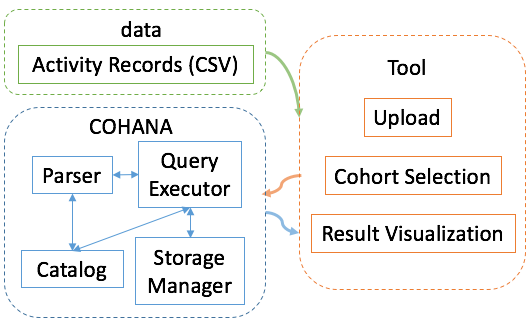
\includegraphics[width=0.4\textwidth]{arch_tool.png}
    \caption{System Architecture}
    \label{fig:sys_arch}
\end{figure}

Figure \ref{fig:sys_arch} outlines the architecture including three components, i.e., data, Cohana engine and our tool, along with data flow among the components.

The only data we required is a CSV file of user activity records, including indispensable columns of User ID, event, and time for a cohort definition. The dataset should be sorted by user id, and the records for a single user are sorted chronologically, which facilitates finding the birth activity tuple. It is a ubiquitous format for data analysis, especially for cohort analysis, and reasonably simple to achieve once and for all.

The Cohana engine consists of parser, catalog, query executor and storage manager, wherein the last two are the cores to support efficient cohort queries. The storage manager applies a chunking scheme and a series of compression techniques. To be more specific, we partition the data into chunks horizontally where every chunk stores precisely activity tuples of one user. Afterwards, different compression schemes are employed on columns regarding their types, i.e., Run-Length-Encoding for user identity column, two-level compression in global and chunk respectively for string column and delta encoding scheme for integer column. On the other hand, the query executor generates a logical query plan in the form of operator tree from the original cohort query and optimize by birth selections. After being executed on each data chunk in the storage manager, the query plan merges and presents the results.

The tool for cohort analysis systems, implemented under Django framework, is responsible for all front-end user interactions such as loading data, composing queries, and displaying visualized results, and back-end data connections and operations such as communicating with cohort analysis engines. As long as the user specifies the dataset on the web interface, the tool will compose and send it to the Cohana engine, and extract the column information for options in cohort analysis page. The tool structures the birth event, cohort selection, and age in a natural-language way, such that users can map their requirements into the options with ease. After that, the options selected are translated into JSON file in the format requested by Cohana engine. Finally, the result is sent back, parsed and visualized on the web page.

\section{Demonstration Outlines}

We will walk through the whole system on the medical example in the Introduction section to illustrate the usage of our tool for cohort analysis. It's worth mentioning that an example in medical area though it is, such analysis is common in any domain and could be elegantly handled by our tool.

\subsection{Data Preparation}

For the sake of confidentiality, the data we use for the demo are generated according to the schema of real health care data, while complying with the distributions in the original one to be as representative as possible. We have eight columns in the CSV dataset, i.e., \emph{id, birthyear, event, disease, medicine, labtest, value, and time}. \emph{id} is a unique identifier for each patient, and \emph{birthyear} and \emph{time} are unambiguous. The three options---diagnose, prescribe and labtest---in the \emph{event} column state the actions of users, while the \emph{disease}, \emph{medicine}, and \emph{labtest} columns specify details for them respectively. The \emph{disease} column contains a particular code for the illness diagnosed when a patient is admitted if the \emph{event} is diagnose, or a default value otherwise. When a patient is in the hospital for more than one day, he might have only one record of diagnose for the whole visit. The \emph{medicine} column indicates the prescription issued to the patient and surely might not cover all days during his visit. The \emph{labtest} means the type of test patients take and the \emph{value} declares the integral test result. For example, \ref{fig:upload} shows that the patient P-0 was admitted to the hospital on 1st January 2012, diagnosed with Disease-B, prescribed Medicine-C, and got 44 on Labtest-C. On the next day, he got 25 on the same lab test. We notice the redundancy in the records, but it is common for applications wherein tables integrated by many sub-tables, and the storage manager in the Cohana engine will compress them intelligently to assure low storage consumption and high query efficiency, provided the User ID, event and time columns.

% \begin{figure}
% \begin{subfigure}{.5\textwidth}
%   \centering
%   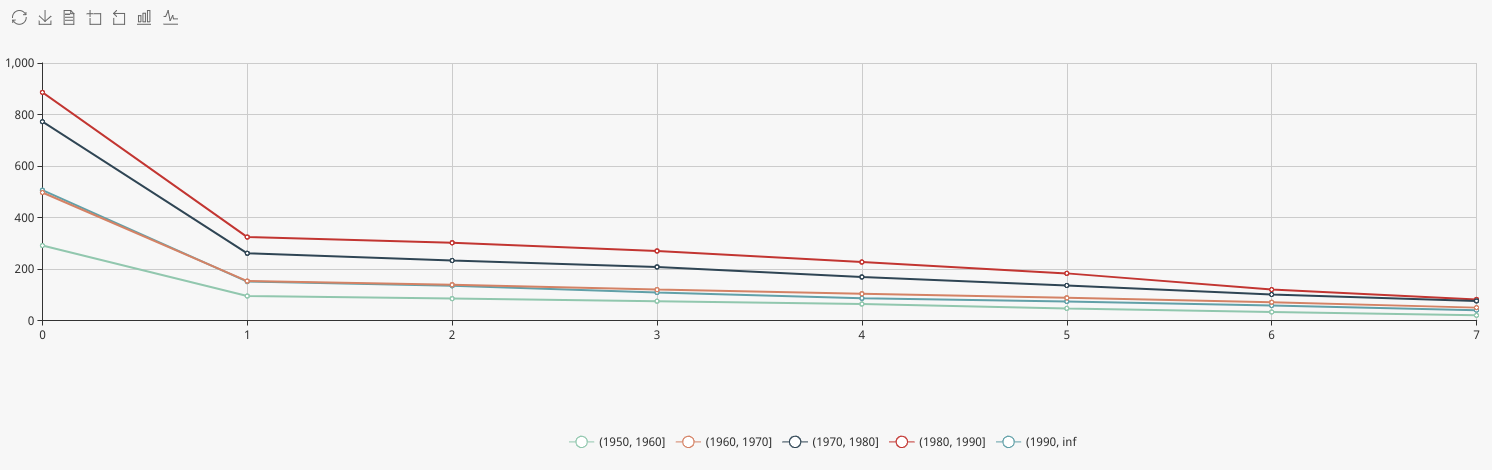
\includegraphics[width=.8\linewidth]{image1}
%   \caption{1a}
%   \label{fig:sfig1}
% \end{subfigure}%
% \begin{subfigure}{.5\textwidth}
%   \centering
%   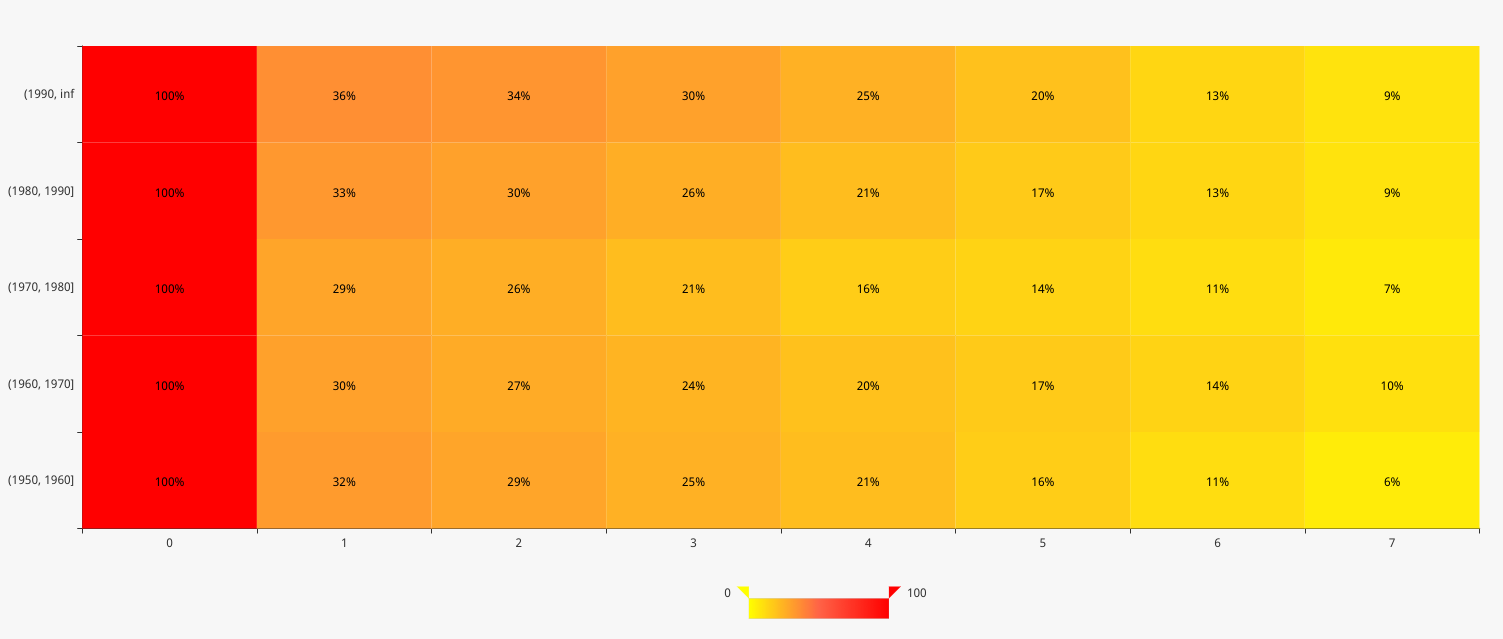
\includegraphics[width=.8\linewidth]{image2}
%   \caption{1b}
%   \label{fig:sfig2}
% \end{subfigure}
% \caption{plots of....}
% \label{fig:fig}
% \end{figure}

\begin{figure*}
\begin{subfigure}{0.3\textwidth}
    \centering
    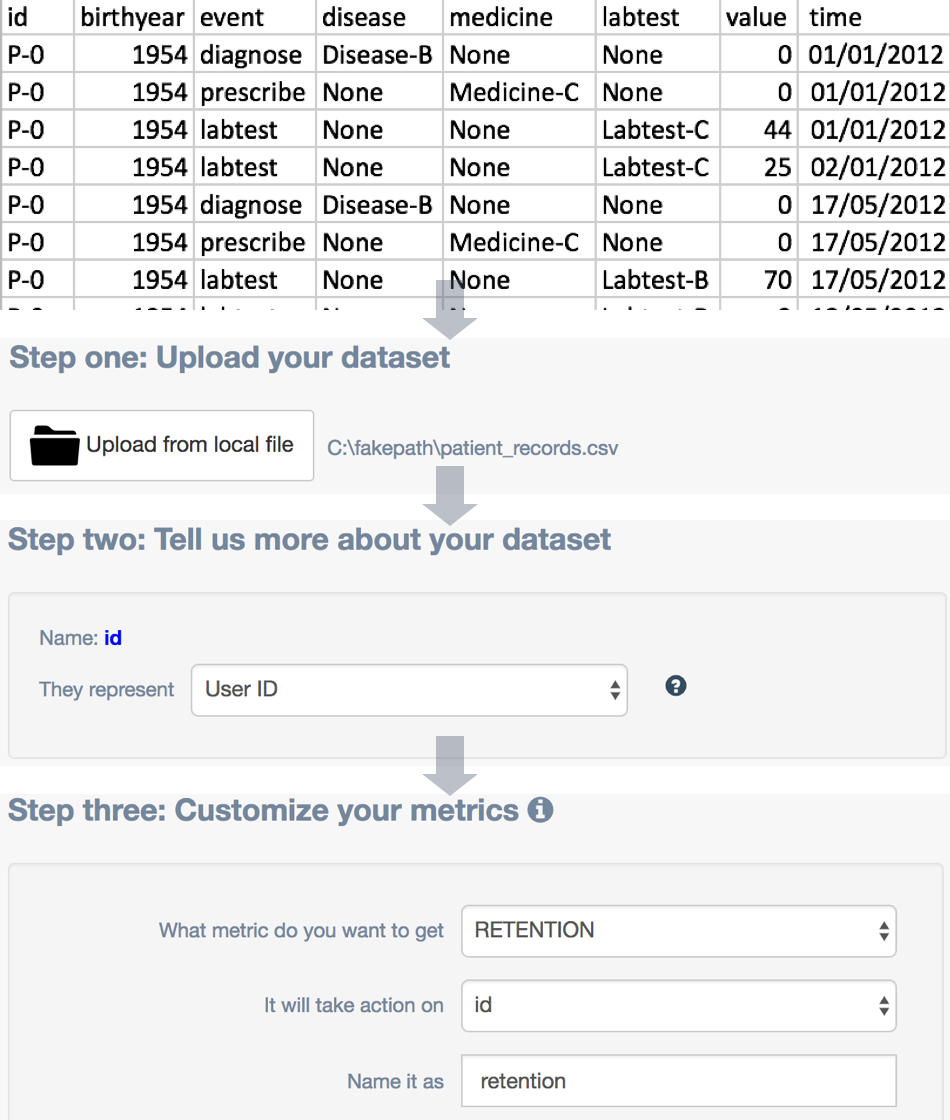
\includegraphics[width=0.9\linewidth]{upload_all_vertical.png}
    \caption{Data Upload}
    \label{fig:upload}
\end{subfigure}%
\begin{subfigure}{0.4\textwidth}
    \centering
    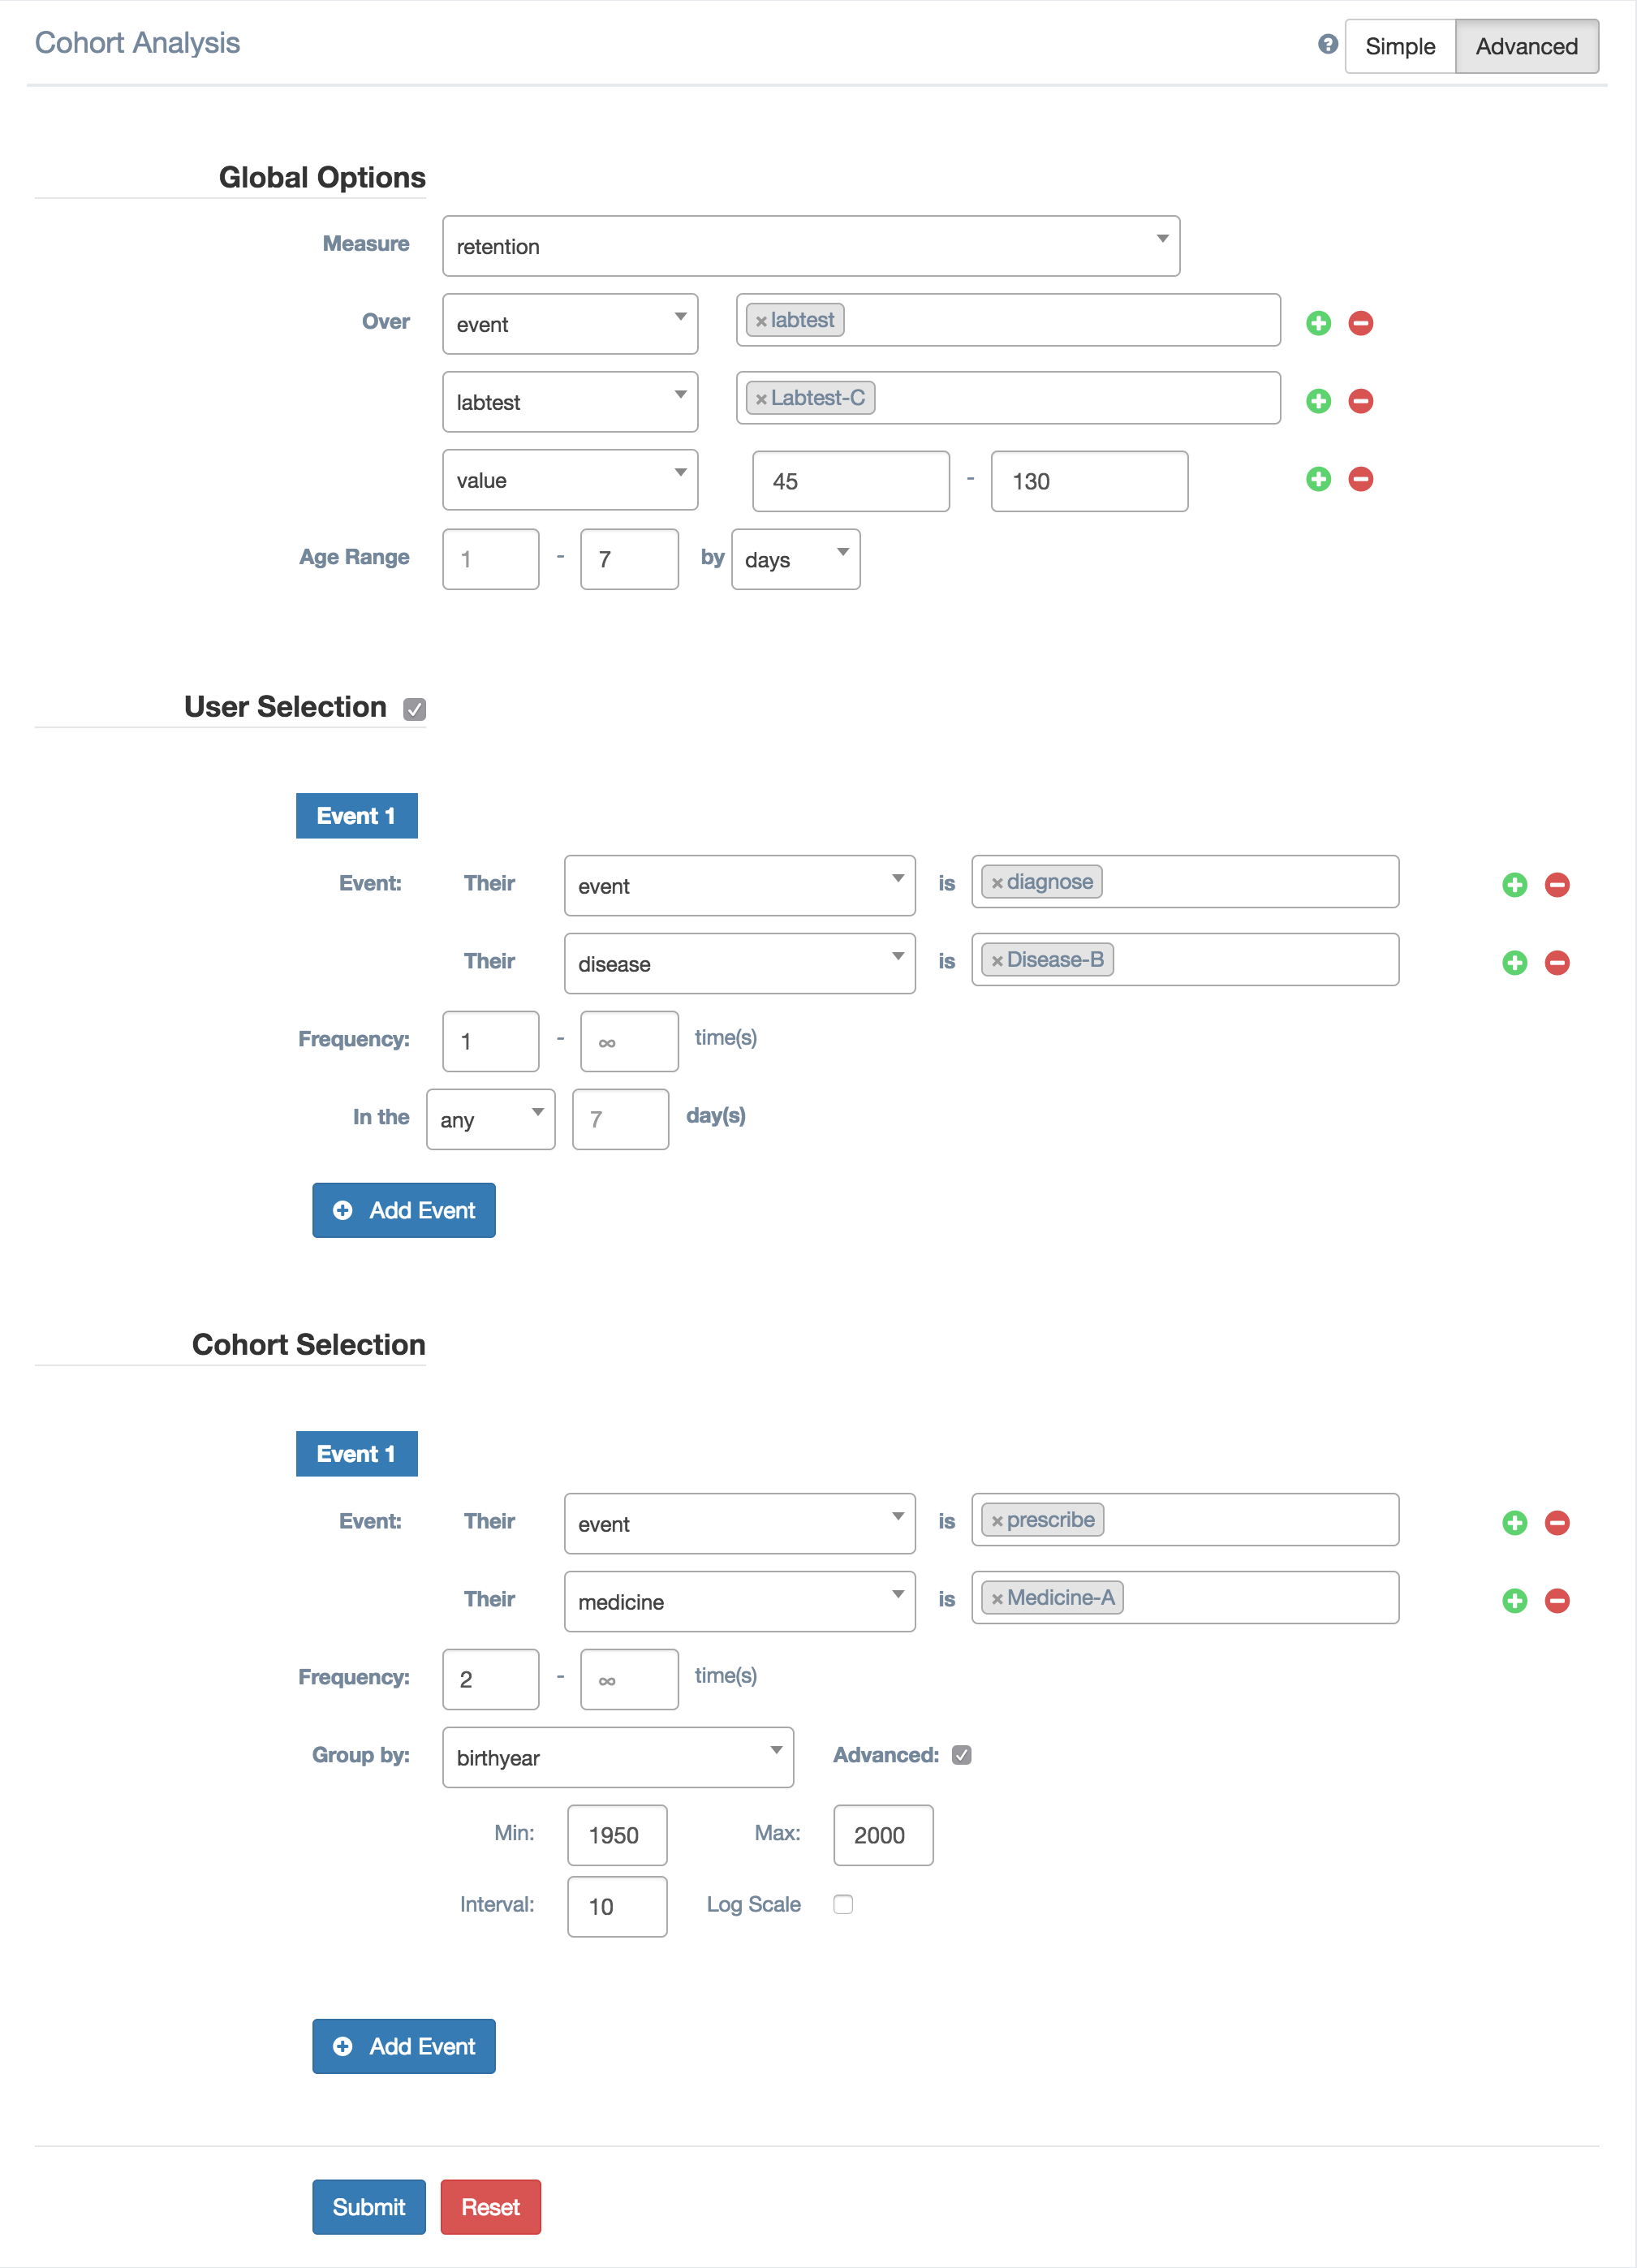
\includegraphics[width=0.9\linewidth]{query.png}
    \caption{Cohort Selection}
    \label{fig:cohort}
\end{subfigure}%
\begin{subfigure}{0.3\textwidth}
    \centering
    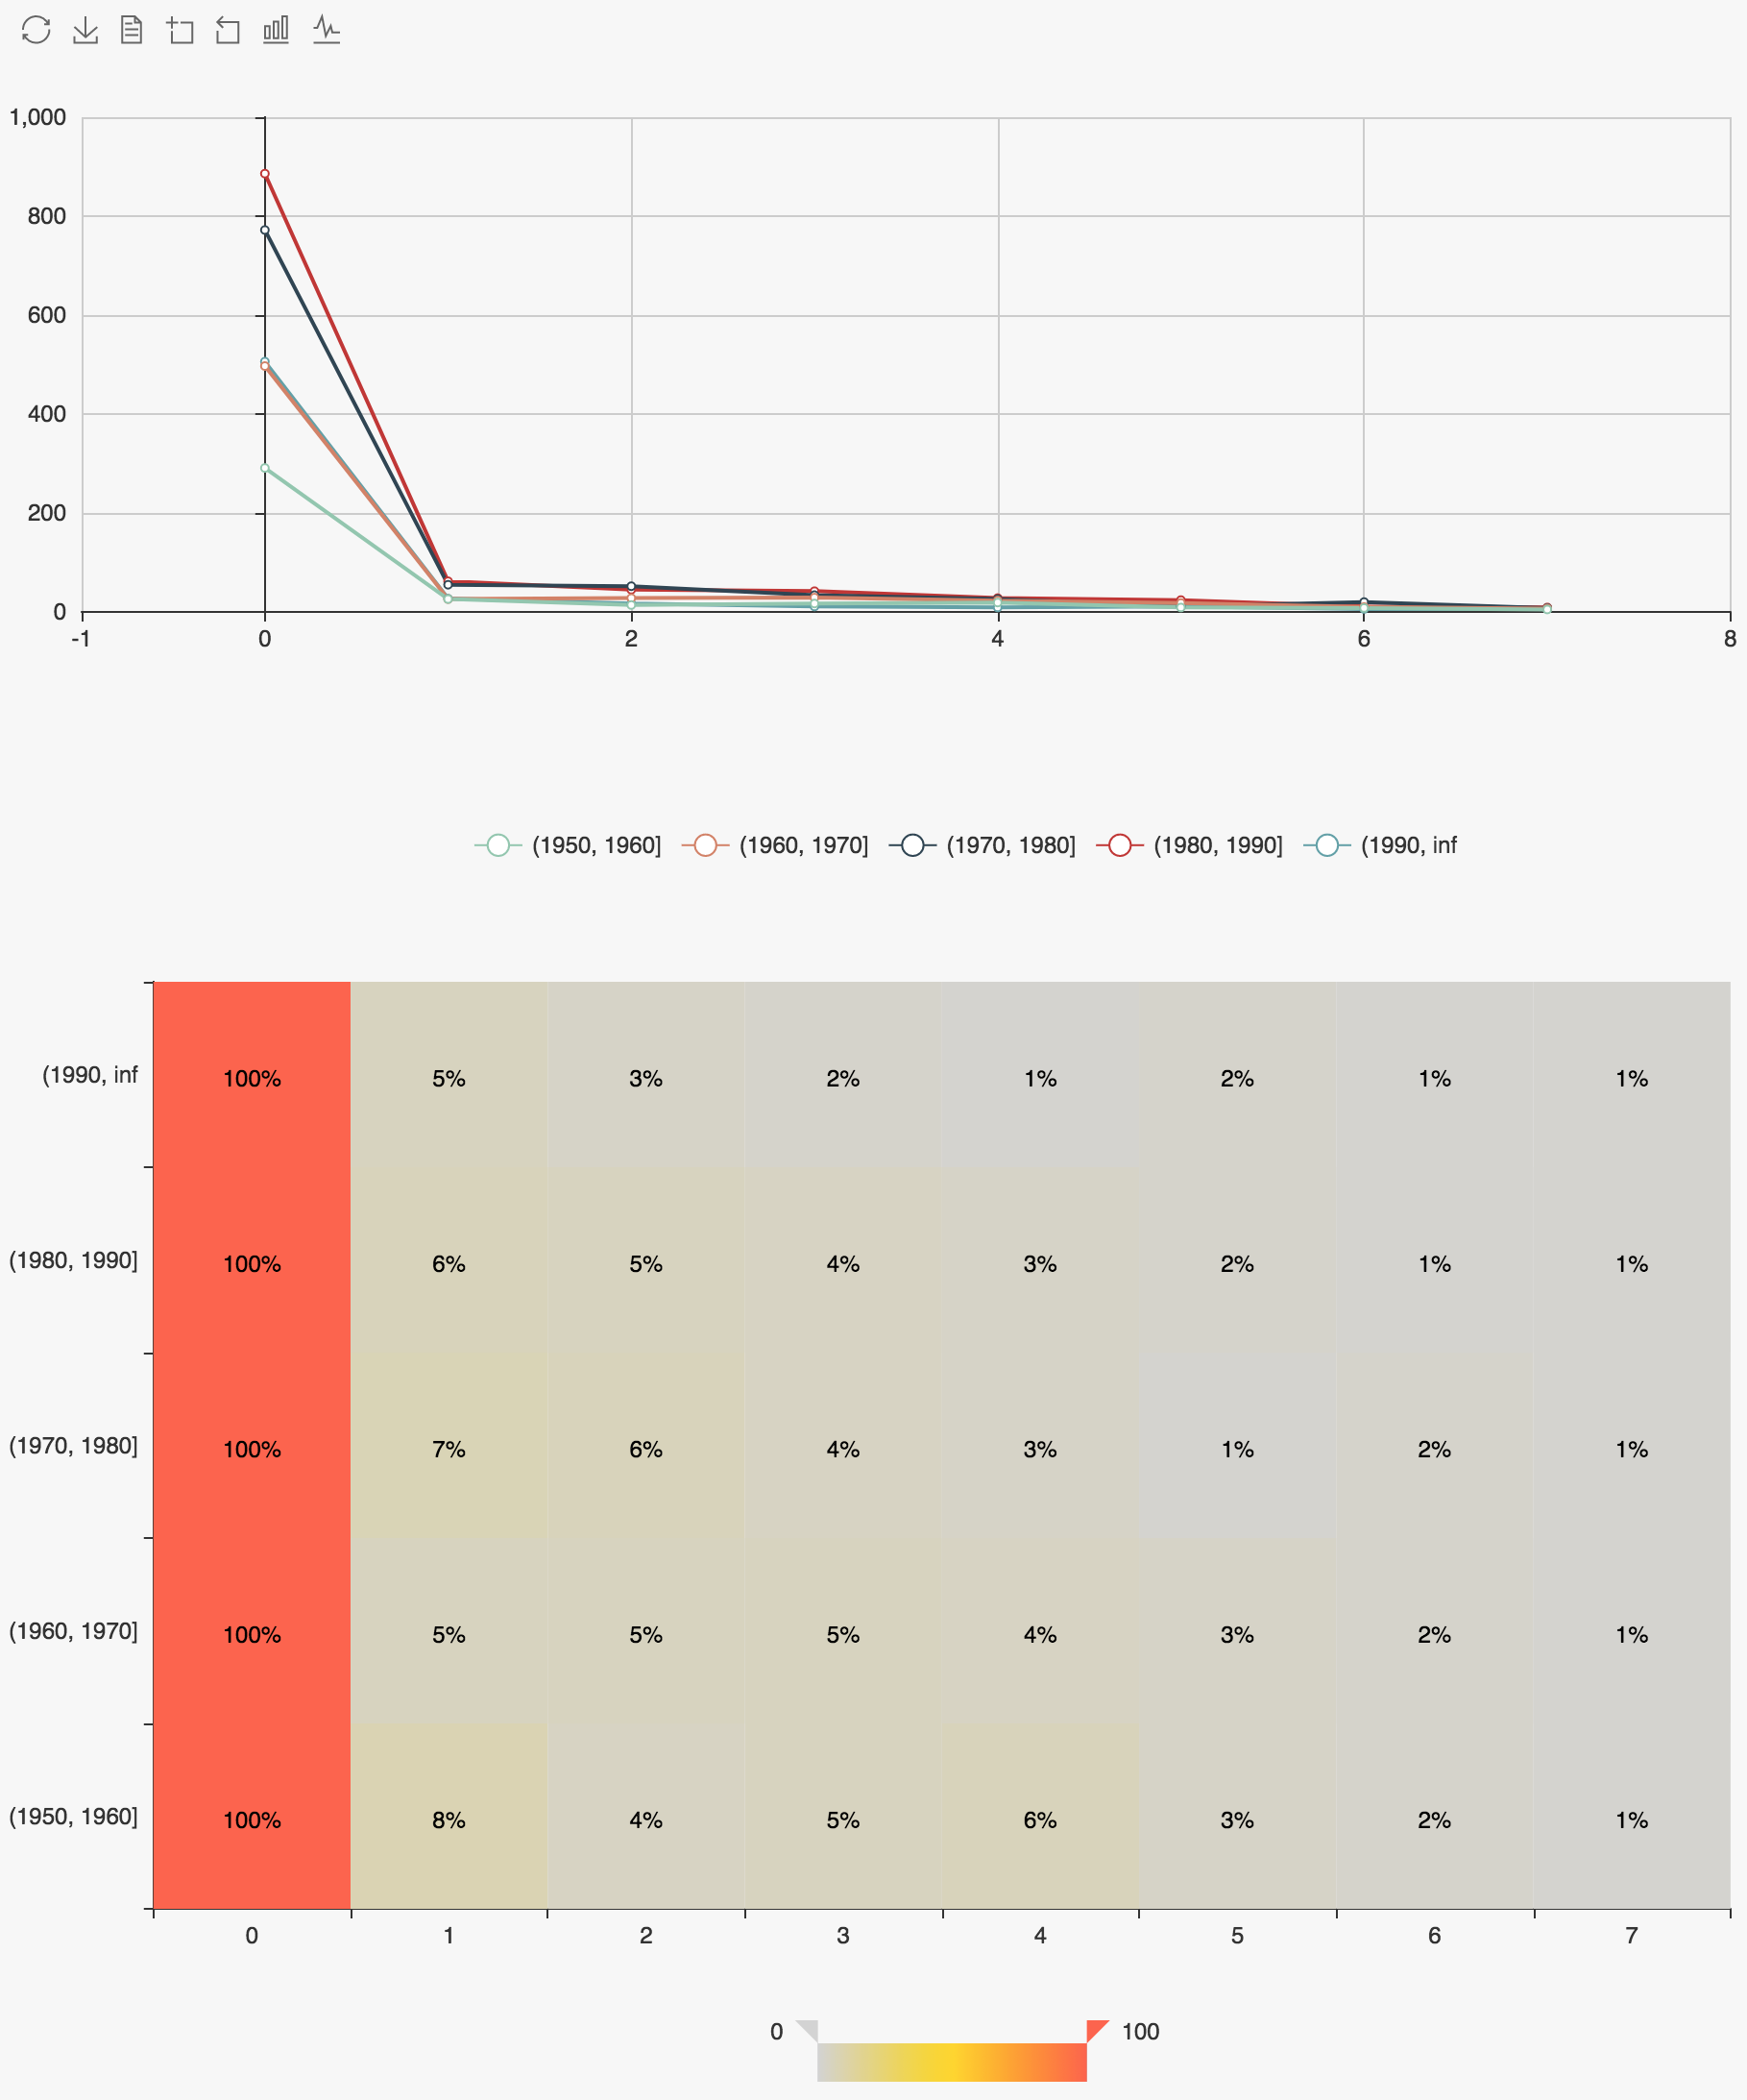
\includegraphics[width=0.9\linewidth]{chart.png}
    \caption{Result Visualization}
    \label{fig:visual}
\end{subfigure}%
\caption{Web Interface}
\end{figure*}

\begin{table}[h!]
\begin{center}
    \begin{tabular}{ |c|c| }
        \hline
        Options & Description \\[0.5ex] 
        \hline\hline
        User ID & user identity \\
        \hline
        Event & action the user performs\\
        \hline
        Event Related & other string columns\\
        \hline
        Value & other integer columns\\
        \hline
        Time & action time \\
        \hline
    \end{tabular}
\end{center}
\caption{Schema Selection for the Dataset}
\label{table:schema}
\end{table}

\begin{table}[h!]
\begin{center}
    \begin{tabular}{ | c | c | }
        \hline
        Options & Description \\[0.5ex] 
        \hline\hline
        RETENTION & number of users \\
        \hline
        COUNT & number of records \\
        \hline
        SUM & sum of certain integer column \\
        \hline
    \end{tabular}
\end{center}
\caption{Metrics Selection for the Dataset}
\label{table:metrics}
\end{table}

The first step we need to do on the web page is to upload the CSV file and specify the schema and metrics as shown in Figure \ref{fig:upload}. The descriptions for options of schema and metrics are shown in \ref{table:schema} and \ref{table:metrics}. Obviously, we choose RETENTION for our metrics for the problem, meaning the number of patients eligible in each cohort and age since their birth. Of course we can choose COUNT on labtest if we want to count the number of abnormal values, or SUM if we need to inspect the exact abnormal values. The tool allows assigning multiple metrics. As long as the Cohana engine receives the file and specification, the web page navigates us to the Cohort Analysis page where options are equipped with the content in the records.

\subsection{Cohort Selection}

% \begin{figure}
%     \centering
%     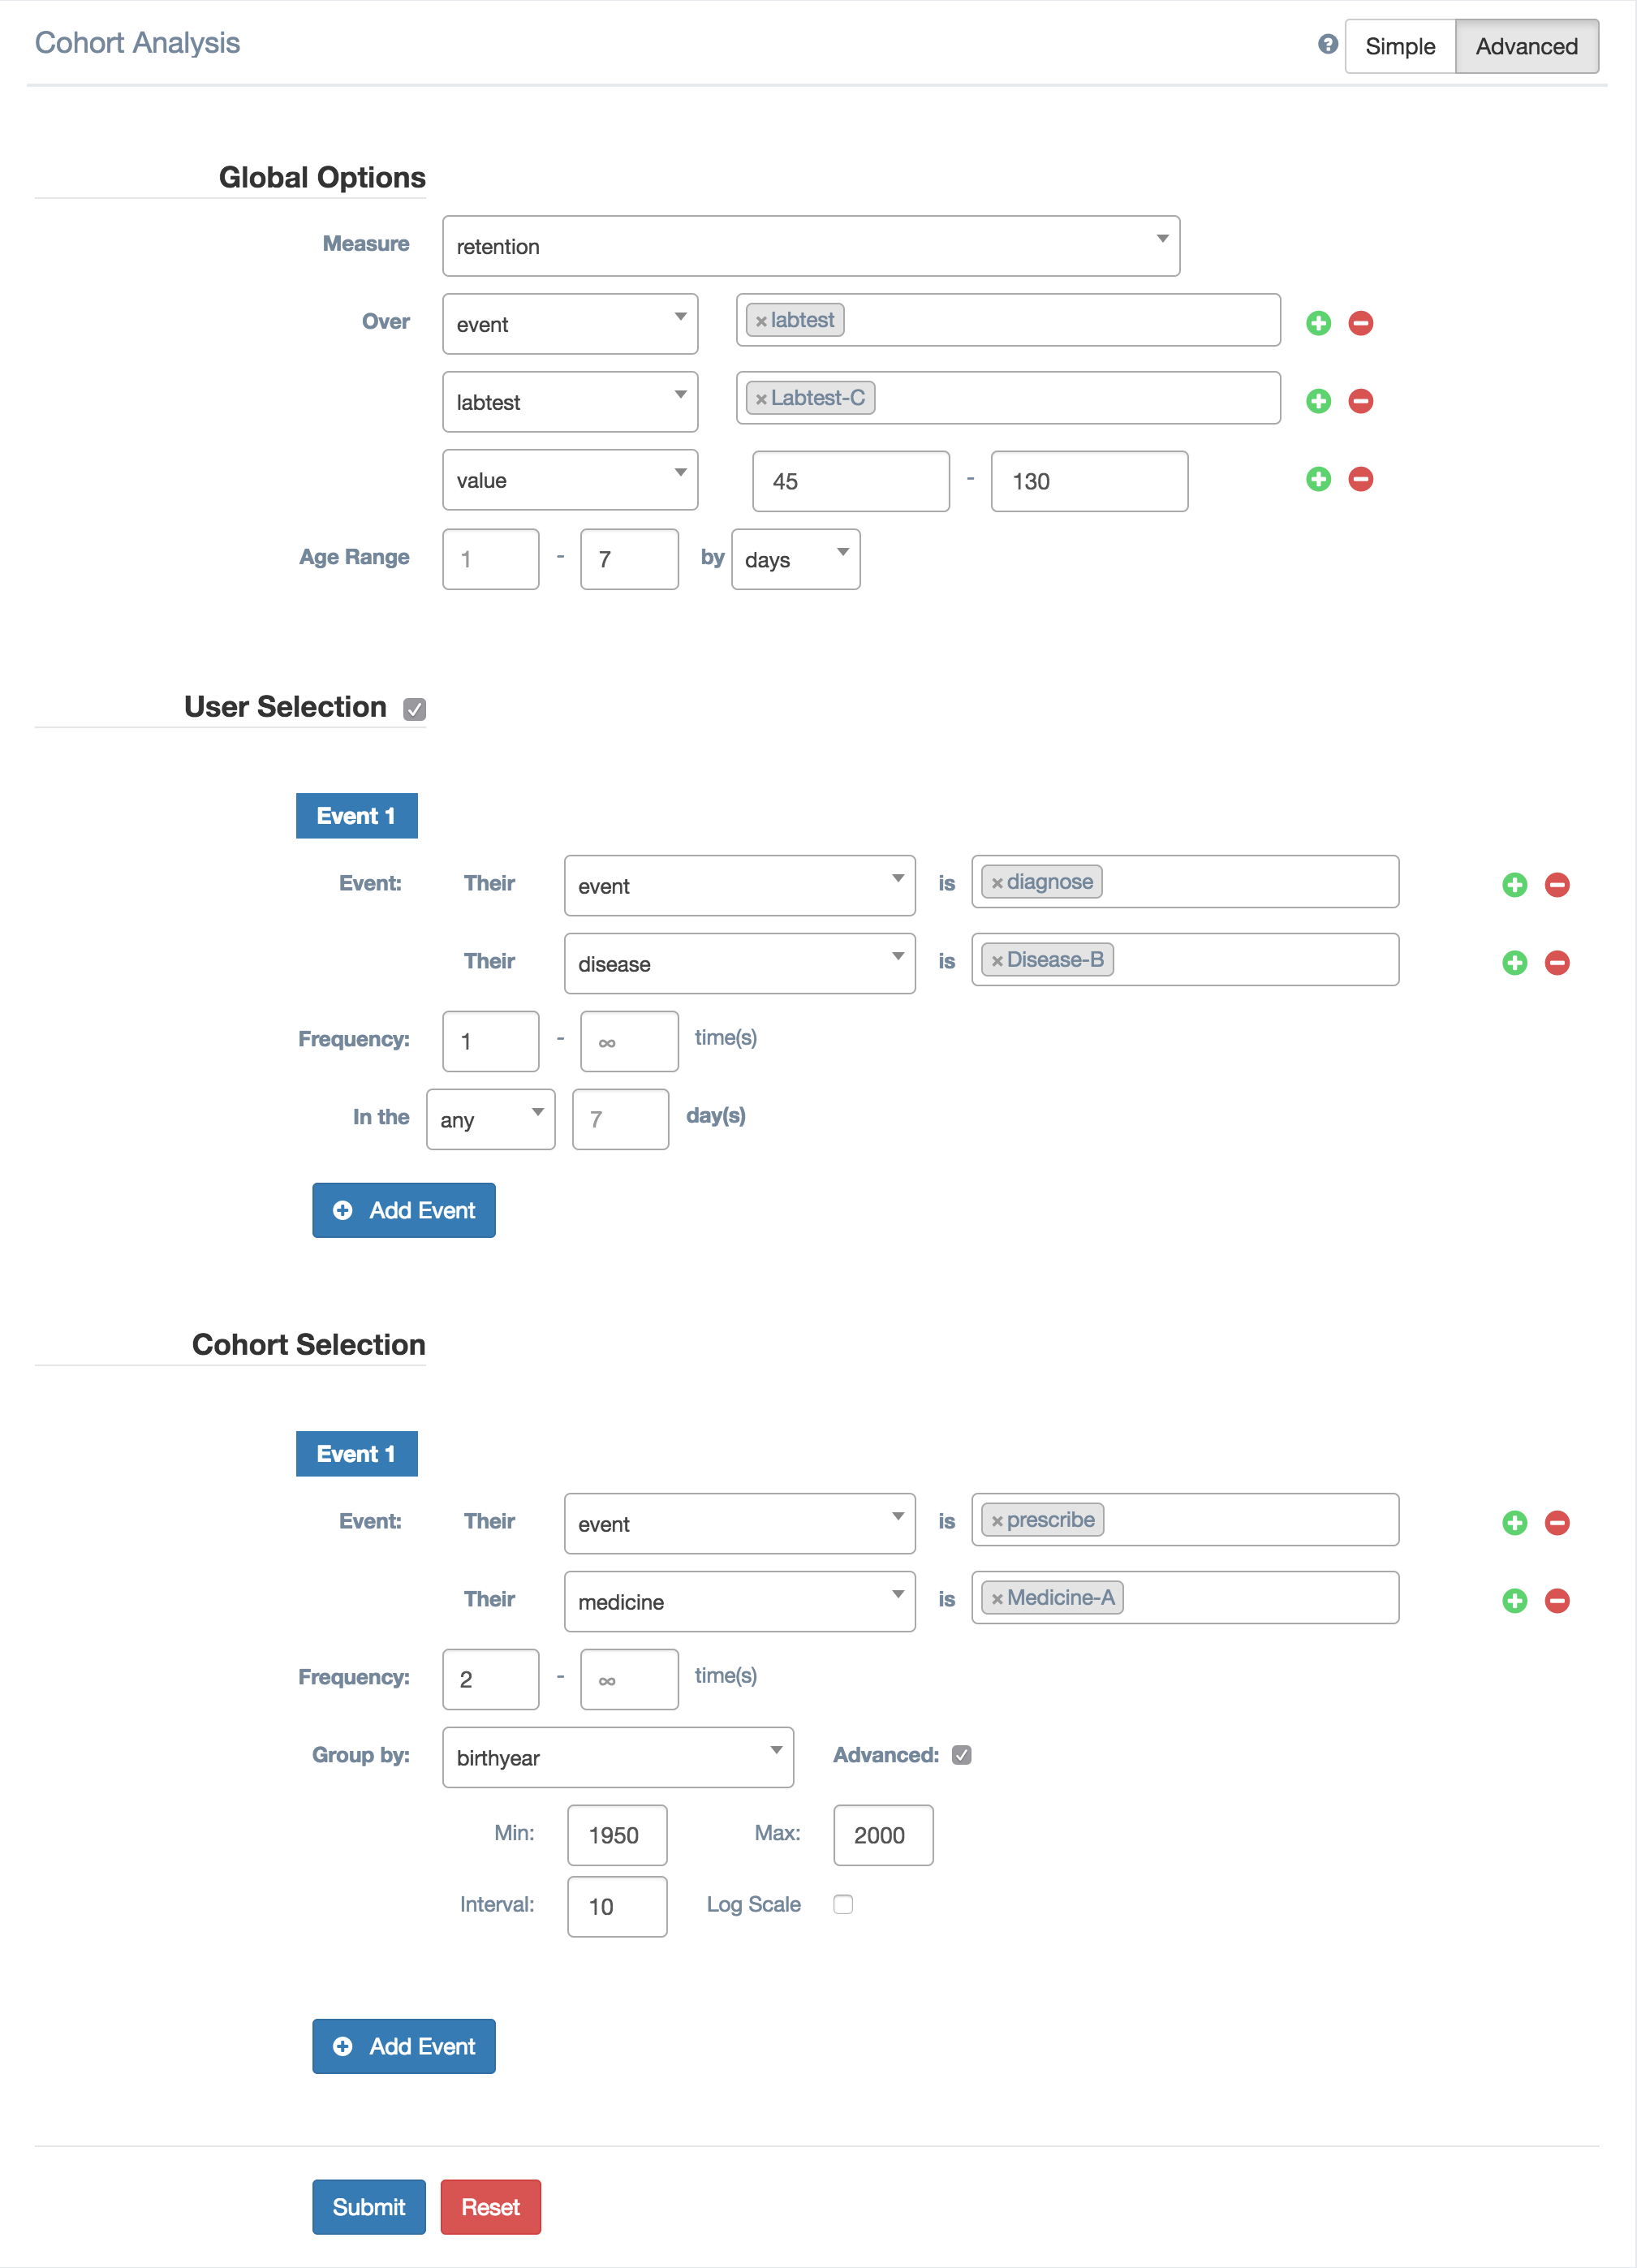
\includegraphics[width=0.45\textwidth]{query.png}
%     \caption{Cohort Selection}
%     \label{fig:query}
% \end{figure}

According to the example, 1) we consider only patients who have disease B; 2) the birth event is taking medicine A two times; 3) the age is one day; 4) we aggregate by the count of abnormal values in lab-test C since birth. Following the decomposition of the requirement, the only thing we need to do is to fit the sub-requirements into our cohort options on the web page. 

As dipected in \ref{fig:cohort}, in the Cohort Metrics, we measure the \emph{retention} defined in the last step over \emph{event is labtest} and \emph{labtest is Labtest-C} that \emph{valued 45 to 130} where \emph{age range is 1 to 7 days}. The age range settles the period we investigate after users' birth, i.e., small range for short-term effect and large range for long-term effect. The next selection is on user which can be unchecked if we conduct on all users. Under our context, we choose \emph{Their event is diagnose} and \emph{Their disease is Disease-B} while leaving the frequency with the default value in \emph{any 7 days}. We can cast more constraints on the records, such as \emph{Their time is 2015-01-01 - 2015-12-31} to analyze the data in 2015 only, by ticking the \textbf{+} button on the right. In the Birth Criteria, we realize the birth event by selecting \emph{Their event is prescribe} and \emph{Their medicine is Medicine-A} and the frequency to be \emph{2-$\infty$ times}. If multiple birth events are assigned by ticking the \textbf{+} button, a patient is regarded born only when all the birth events are met. Finally we \emph{Group by birthyear} in the range of \emph{1950 to 2000 scaled 10}, meaning we group the patients by decade.

\subsection{Result Visualization}

Within seconds of submitting the requirement, a line chart and a heatmap chart of cohort analysis result (\ref{fig:visual}) will be displayed under the cohort options. In the line chart, the x-axis represents the \emph{age} of patients since birth——--days after taking two times of Medicine A in our context---and y-axis represents the aggregated result, i.e., the number of patients detected abnormal in the Labtest-C. Values of age 0 are the numbers of patients born. Each line stands for a group of patients in the different birth years. The line chart, answering the cohort query numerically, not only illustrates the trend of user behavior in various groups along the time but offers a sharp contrast of behavior among groups. The other 2-D heatmap chart is axised with age and group. Each block in the chart accounts for the proportion of patients living up to the cohort conditions in that group and age compared to those when born. The first column, on behalf of age 0, is sure to value 100\%. The blocks with different color depths give spontaneous expression to the relationship between age and user behavior and may indicate deeper insights on the user behavior of the different groups. The two charts explain the data in absolute and relative way respectively. For example, more young patients are active on the side effect, suggested by the high values in the line chart, while elder patients take longer to be accustomed to medicine as the color retains deep in the heatmap chart.

What's more, we provide a wide variety of operations on the chart such as zooming in and changing the chart type, as shown in the toolbar above the chart, with the help of a third-party library. These functions afford immediate responses to visualization exploration, helpful for further data excavation.

\section{Related Work and Conclusion}

MixPanel. Amplitude. 

The demonstration shows a powerful and comprehensive tool for cohort analysis while keeping the operations as simple and intuitive as possible. Benefit from ultra efficiency of Cohana engine, the users can conduct report or verify their ideas in no time. Besides, the three cohort definitions, though concise, covers a broad range of practical data analysis needs in various domains. Further, the rich chart operations provide better understanding and deeper insight towards user behavior.

%\section*{Acknowledgment}



\bibliographystyle{IEEEtran}

\bibliography{ref_list}

\end{document}
